\subsubsection{Mô hình cho tập dữ liệu chỉ bao gồm các quan sát có cột "emailtotal" chỉ là giá trị null}


\begin{enumerate}[label=(\alph*)]
    \item Đầu vào mô hình là vector thu được từ phân tích thành phần chính sử dụng thuật toán PCA
    
    Ta có bảng kết quả huấn luyện mô hình:

    \begin{python}
                    precision    recall  f1-score   support

   Keeping house       0.00      0.00      0.00        55
           Other       0.25      0.04      0.07        23
         Retired       0.37      0.48      0.42       113
          School       0.00      0.00      0.00        13
Temp not working       0.00      0.00      0.00         8
Unempl, laid off       0.00      0.00      0.00        19
Working fulltime       0.49      0.73      0.58       198
Working parttime       0.14      0.04      0.06        55

        accuracy                           0.42       484
       macro avg       0.16      0.16      0.14       484
    weighted avg       0.31      0.42      0.35       484
    \end{python}

    và ma trận nhầm lẫn:

    \begin{figure}[H]
        \centering
        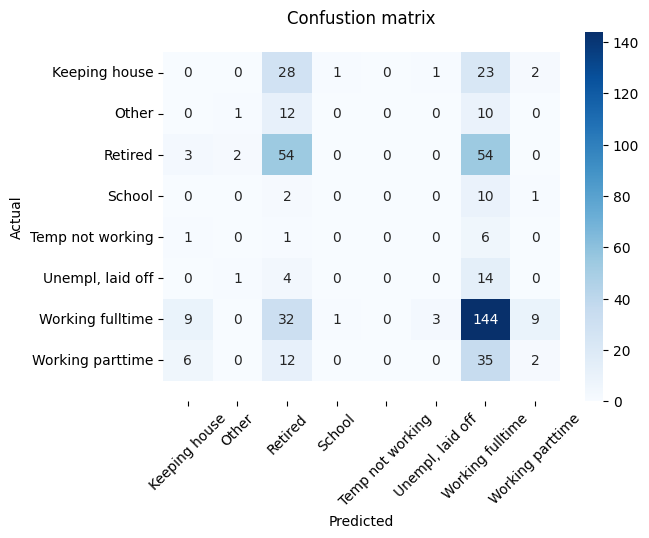
\includegraphics[width=0.6\textwidth]{figures/Thanh/Models/XGBoost/With_null_models_confusion_matrix_XGBoost_PCA_features.png}
        \caption{Ma trận nhầm lẫn của mô hình XGBoost khi vector đầu vào được phân tích thành phần chính}
        \label{fig:With_null_models_confusion_matrix_XGBoost_PCA_features}
    \end{figure}

    Ta nhận thấy kết quả độ chính xác không tốt như trường hợp sử dụng mô hình AdaBoost
    

    Ta sẽ phân tích ngược trở lại trọng số của các tham số tương ứng với các đặc trưng của vector ban đầu từ các tham số ứng với các đặc trưng của các thành phần chính:

    \begin{figure}[H]
        \centering
        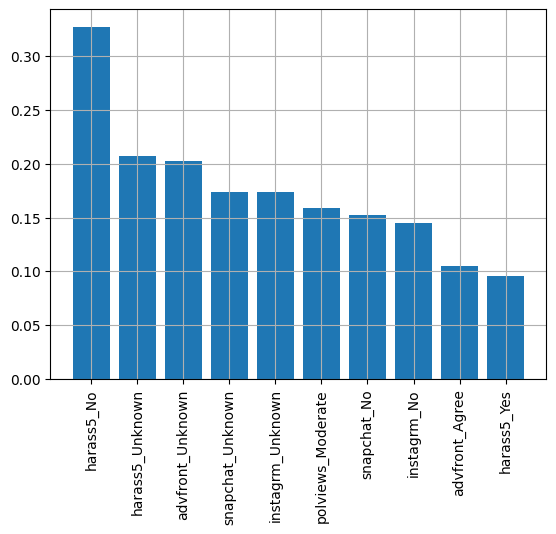
\includegraphics[width=0.6\textwidth]{figures/Thanh/Models/XGBoost/With_null_models_Feature_Importance_XGBoost_PCA_features.png}
        \caption{Biểu đồ cột sắp xếp độ lớn giảm dần (trị tuyệt đối) tham số của các đặc trưng}
        \label{fig:With_null_models_Feature_Importance_XGBoost_PCA_features}
    \end{figure}

    Ta có biểu đồ cột sắp xếp độ lớn giảm dần (trị tuyệt đối) tham số của các đặc trưng thể hiện ở hình \ref{fig:With_null_models_Feature_Importance_XGBoost_PCA_features}.
    Ta nhận thấy các cột có trọng số lớn và ảnh hưởng nhiều tới các các nhãn đầu ra là harass5\_No và harass5\_Unknown.
    Cả hai đặc trưng trên đều có tần suất xuất hiện lớn trong tập dữ liệu.

    \item Vector đầu vào là vector gốc ban đầu
    
    Ta có bảng kết quả huấn luyện mô hình:

    \begin{python}
                    precision    recall  f1-score   support

   Keeping house       0.18      0.04      0.06        55
           Other       0.00      0.00      0.00        23
         Retired       0.40      0.53      0.46       113
          School       0.00      0.00      0.00        13
Temp not working       0.00      0.00      0.00         8
Unempl, laid off       0.00      0.00      0.00        19
Working fulltime       0.52      0.82      0.64       198
Working parttime       0.38      0.09      0.15        55

        accuracy                           0.48       484
       macro avg       0.19      0.19      0.16       484
    weighted avg       0.37      0.48      0.39       484

    \end{python}

    và ma trận nhầm lẫn:

    \begin{figure}[H]
        \centering
        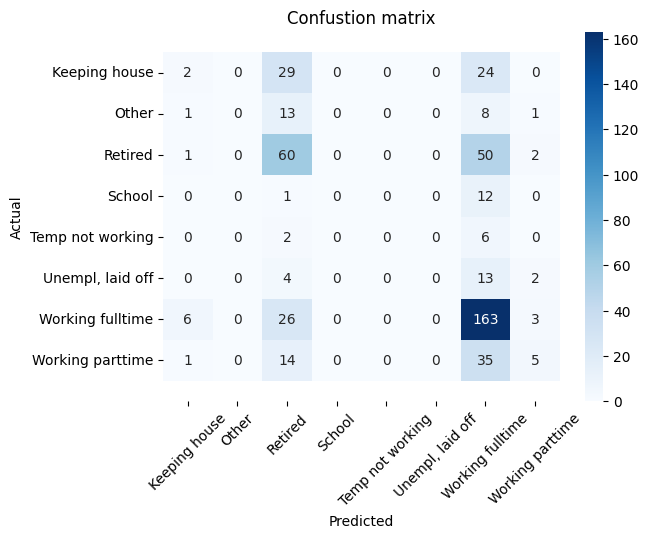
\includegraphics[width=0.6\textwidth]{figures/Thanh/Models/XGBoost/With_null_models_confusion_matrix_XGBoost_original_features.png}
        \caption{Ma trận nhầm lẫn của mô hình XGBoost khi vector đầu vào là vector gốc ban đầu}
        \label{fig:With_null_models_confusion_matrix_XGBoost_original_features}
    \end{figure}

    Ta nhận thấy kết quả dự đoán của mô hình tốt hơn so với các mô hình trước.
    Khi mà nhóm làm việc toàn thời gian có kết quả ngang băng các mô hình trước,
    nhãn Retired và nhãn Working parttime tốt hơn các mô hình khác.
    Chỉ số F1 trung bình cũng cao hơn các mô hình trước
    
    Ta sẽ phân tích ngược trở lại trọng số của các tham số tương ứng với các đặc trưng của vector ban đầu từ các tham số ứng với các đặc trưng:

    \begin{figure}[H]
        \centering
        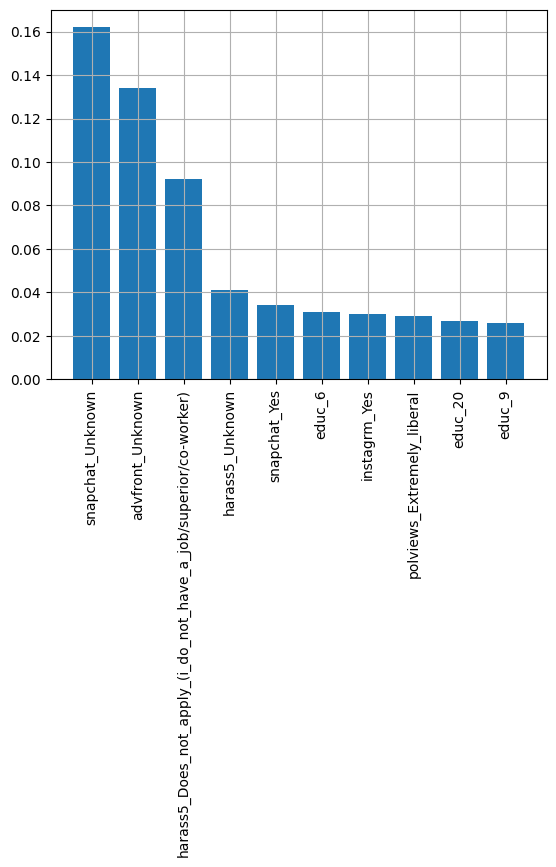
\includegraphics[width=0.6\textwidth]{figures/Thanh/Models/XGBoost/With_null_models_Feature_Importance_XGBoost_original_features.png}
        \caption{Biểu đồ cột sắp xếp độ lớn giảm dần (trị tuyệt đối) tham số của các đặc trưng (mô hình với vector đầu vào là vector gốc ban đầu)}
        \label{fig:With_null_models_Feature_Importance_XGBoost_original_features}
    \end{figure}
    
    Ta có biểu đồ cột sắp xếp độ lớn giảm dần (trị tuyệt đối) tham số của các đặc trưng thể hiện ở hình \ref{fig:With_null_models_Feature_Importance_XGBoost_original_features}.
    Ta nhận thấy các đặc trưng có trọng số lớn tương ứng với các đặc trưng là snapchat\_Unknown và advfont\_Unknown.
    Hai đặc trưng này có tần suất xuất hiện rất nhiều trong tập dữ liệu
\end{enumerate}